% Created by tikzDevice version 0.12.6 on 2024-01-30 13:47:14
% !TEX encoding = UTF-8 Unicode
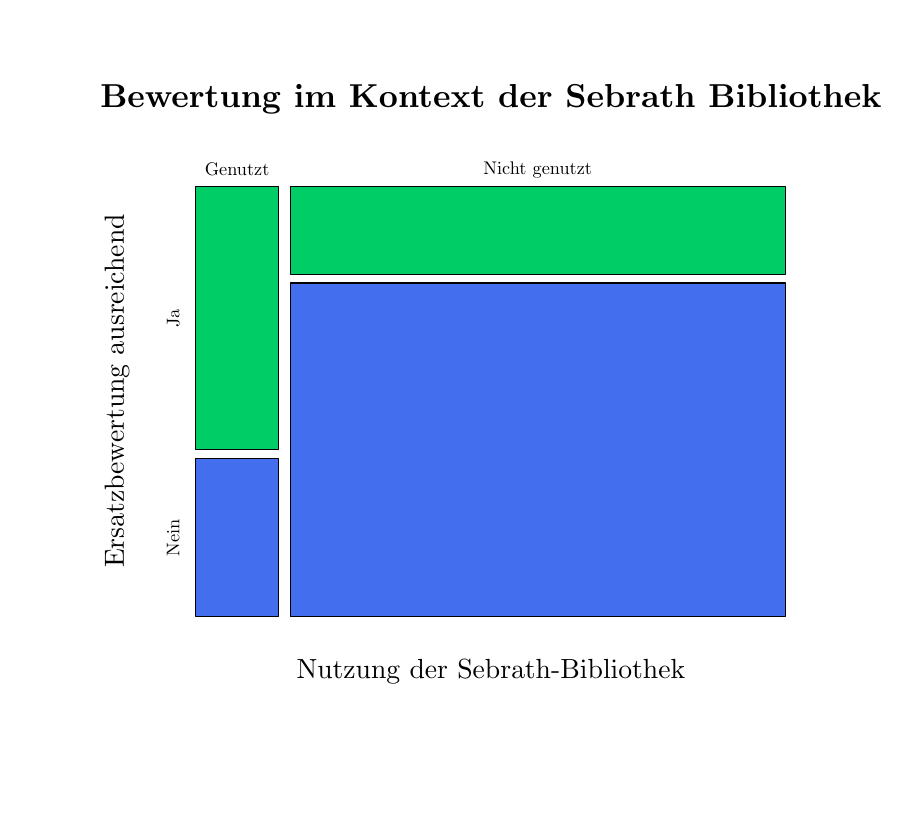
\begin{tikzpicture}[x=1pt,y=1pt]
\definecolor{fillColor}{RGB}{255,255,255}
\path[use as bounding box,fill=fillColor,fill opacity=0.00] (0,0) rectangle (310.76,274.63);
\begin{scope}
\path[clip] (  0.00,  0.00) rectangle (310.76,274.63);
\definecolor{drawColor}{RGB}{0,0,0}

\node[text=drawColor,anchor=base,inner sep=0pt, outer sep=0pt, scale=  1.20] at (167.38,245.89) {\bfseries Bewertung im Kontext der Sebrath Bibliothek};

\node[text=drawColor,anchor=base,inner sep=0pt, outer sep=0pt, scale=  1.00] at (167.38, 39.60) {Nutzung der Sebrath-Bibliothek};

\node[text=drawColor,rotate= 90.00,anchor=base,inner sep=0pt, outer sep=0pt, scale=  1.00] at ( 34.80,143.31) {Ersatzbewertung ausreichend};
\end{scope}
\begin{scope}
\path[clip] (  0.00,  0.00) rectangle (310.76,274.63);
\definecolor{drawColor}{RGB}{0,0,0}

\node[text=drawColor,anchor=base,inner sep=0pt, outer sep=0pt, scale=  0.66] at ( 75.70,221.07) {Genutzt};

\node[text=drawColor,anchor=base,inner sep=0pt, outer sep=0pt, scale=  0.66] at (184.30,221.71) {Nicht genutzt};

\node[text=drawColor,rotate= 90.00,anchor=base,inner sep=0pt, outer sep=0pt, scale=  0.66] at ( 54.79,169.63) {Ja};

\node[text=drawColor,rotate= 90.00,anchor=base,inner sep=0pt, outer sep=0pt, scale=  0.66] at ( 54.79, 90.40) {Nein};
\end{scope}
\begin{scope}
\path[clip] ( 49.20, 61.20) rectangle (285.56,225.43);
\definecolor{drawColor}{RGB}{0,0,0}
\definecolor{fillColor}{RGB}{0,205,102}

\path[draw=drawColor,line width= 0.4pt,line join=round,line cap=round,fill=fillColor] ( 60.79,122.06) --
	( 90.60,122.06) --
	( 90.60,217.21) --
	( 60.79,217.21) --
	cycle;
\definecolor{fillColor}{RGB}{67,110,238}

\path[draw=drawColor,line width= 0.4pt,line join=round,line cap=round,fill=fillColor] ( 60.79, 61.86) --
	( 90.60, 61.86) --
	( 90.60,118.95) --
	( 60.79,118.95) --
	cycle;
\definecolor{fillColor}{RGB}{0,205,102}

\path[draw=drawColor,line width= 0.4pt,line join=round,line cap=round,fill=fillColor] ( 94.86,185.49) --
	(273.73,185.49) --
	(273.73,217.21) --
	( 94.86,217.21) --
	cycle;
\definecolor{fillColor}{RGB}{67,110,238}

\path[draw=drawColor,line width= 0.4pt,line join=round,line cap=round,fill=fillColor] ( 94.86, 61.86) --
	(273.73, 61.86) --
	(273.73,182.38) --
	( 94.86,182.38) --
	cycle;
\end{scope}
\end{tikzpicture}
